\subsection{Esybių ir ryšių diagrama}\label{sec:er}

Esybių ir ryšių (ER) diagrama (\ref{fig:er} pav.) parodo, kokius duomenis saugo sistema ir kaip jie tarpusavyje susiję. Diagramos esybės atitinka funkcinių taškų priedo vidinių loginių failų P0.1--P4.1 įrašų tipus (iš viso 24) ir duomenų srautų diagramų saugyklas D1--D9. Grotuvo kopija (D10) į ER neįtraukta, nes ji nėra pagrindinės sistemos duomenų bazės dalis.

Ryšių žymėjimas paaiškintas \ref{tab:er-zymejimas} lentelėje. Ryšys skaitomas pagal ženklus abiejuose linijos galuose, pvz., ryšys tarp Sporto erdvės ir Įrenginio reiškia, kad viena erdvė turi nulį ar daugiau įrenginių, o kiekvienas įrenginys priklauso lygiai vienai erdvei.

\begin{table}[H]
\centering
\caption{ER diagramos ryšių žymėjimas}
\label{tab:er-zymejimas}
\begin{tabular}{|c|l|p{6.5cm}|}
\hline
\textbf{Ženklas} & \textbf{Reikšmė} & \textbf{Pavyzdys} \\
\hline
\texttt{\textbar\textbar} & lygiai vienas & Kiekvienas Užsiėmimas turi lygiai vieną Užsiėmimo nustatymų įrašą. \\
\hline
\texttt{o\textbar} & nulis arba vienas & Naudotojo paskyra turi nulį arba vieną Dalyvio profilį (administratorius profilio neturi). \\
\hline
\texttt{o\{} & nulis ar daugiau & Sporto erdvė turi nulį ar daugiau Įrenginių. \\
\hline
\texttt{\textbar\{} & vienas ar daugiau & Užsiėmimo programa turi bent vieną Programos versiją. \\
\hline
\texttt{*} prie atributo & privalomas atributas & \texttt{* pavadinimas} -- reikšmė būtina. \\
\hline
\texttt{<PK>}, \texttt{<FK>} & pirminis ir išorinis raktas & \texttt{naudotojas\_id <FK>} nurodo į Naudotojo paskyrą. \\
\hline
\end{tabular}
\end{table}

Kai kurių taisyklių ryšių kardinalumas neparodo:
\begin{itemize}
    \item dalyvis viename užsiėmime turi ne daugiau kaip vieną aktyvią rezervaciją;
    \item aktyvių rezervacijų yra ne daugiau nei užsiėmimo vietų;
    \item programa turi tik vieną aktualią versiją;
    \item užsiėmimas iki pradžios vykdo aktualią programos versiją, o prasidėjus versija nebekeičiama;
    \item tuščias užsiėmimo \texttt{treneris\_id} reiškia virtualaus trenerio užsiėmimą (taip pat nurodo atributas \texttt{režimas}), o tuščias vykdymo žurnalo \texttt{treneris\_id} -- ryšio sutrikimo įrašą.
\end{itemize}

Atributo \texttt{būsena} reikšmės atitinka esybių gyvavimo ciklų poskyrį (\ref{tab:er-busenos} lentelė).

\begin{table}[H]
\centering
\caption{ER esybių būsenų reikšmės}
\label{tab:er-busenos}
\begin{tabular}{|l|p{9cm}|}
\hline
\textbf{Esybė} & \textbf{Reikšmės} \\
\hline
Užsiėmimas & suplanuotas, vykdomas, pristabdytas, vykdomas be ryšio, užbaigtas, atšauktas, neįvykęs \\
\hline
Rezervacija & aktyvi, atšaukta, pašalinta \\
\hline
Programos versija & aktuali, ankstesnė \\
\hline
Asmeninė programa & galiojanti, užbaigta, archyvuota \\
\hline
Naudotojo paskyra & aktyvi, neaktyvi \\
\hline
Įrenginys & naudojamas, taisomas, grąžintas \\
\hline
\end{tabular}
\end{table}

\begin{landscape}
\begin{figure}[H]
    \centering
    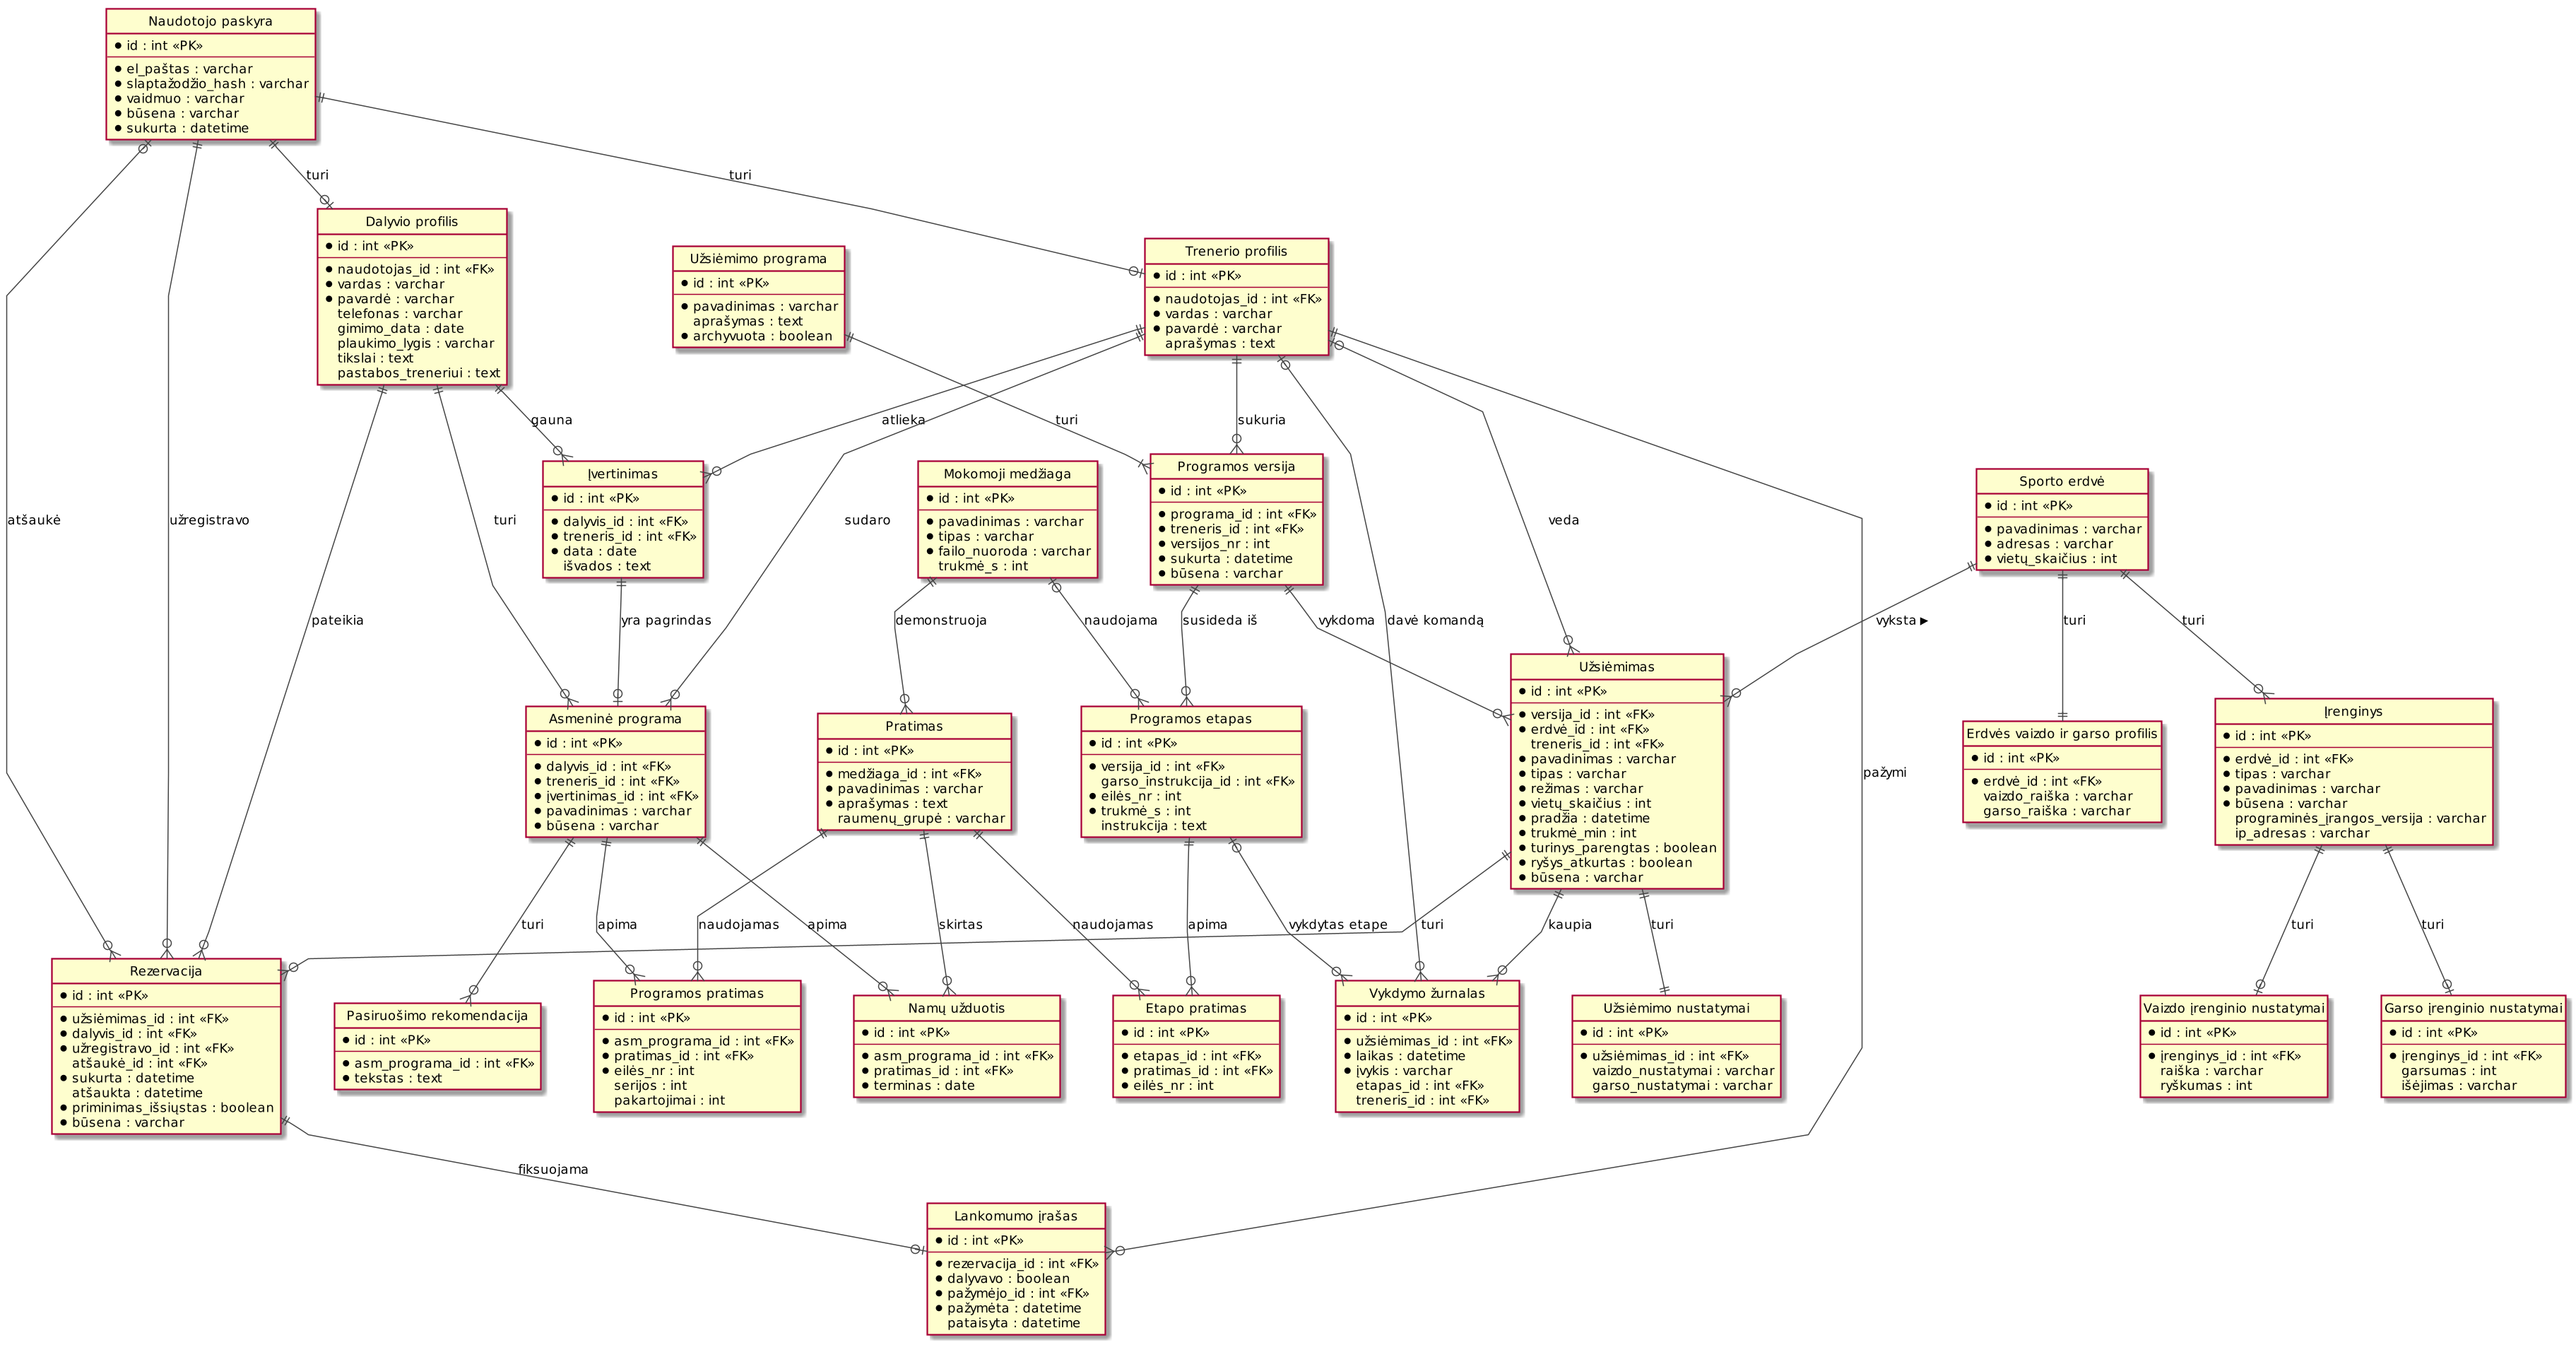
\includegraphics[width=\linewidth,height=0.8\textheight,keepaspectratio]{Struktūrinė analizė/ER diagrama/er_diagrama.png}
    \caption{Esybių ir ryšių diagrama}
    \label{fig:er}
\end{figure}
\end{landscape}